\section*{Transmisiones y Sistemas de Potencia}

\begin{center}
	\begin{tikzpicture}
		\node[inner sep=0pt, rounded corners=10pt] (myimage)
		{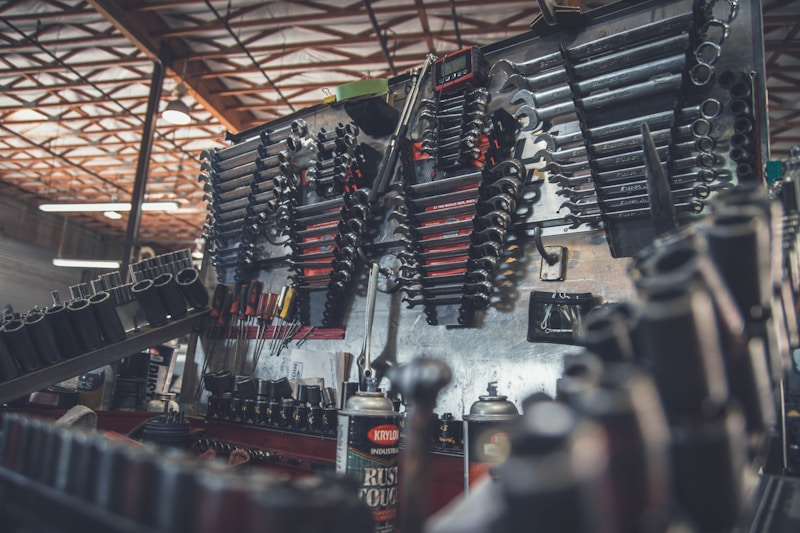
\includegraphics[width=0.6\textwidth,height=6cm]{img/cap3_transmision.jpg}};
	\end{tikzpicture}
\end{center}

El sistema de transmisión es el encargado de canalizar la potencia generada por el
motor hacia las ruedas motrices y la Toma de Fuerza (TDF), permitiendo que el tractor
desarrolle la fuerza de tracción necesaria para las labores agrícolas. Un sistema
robusto y bien mantenido es crucial para operar eficientemente bajo diversas cargas
y terrenos.

\subsection*{Fundamentos de la Transmisión}
La transmisión transforma el alto régimen de giro y bajo torque del motor en una
salida de bajo régimen y alto torque en las ruedas. Este proceso involucra una
serie de engranajes, embragues y ejes que deben trabajar bajo condiciones de alta
presión y temperatura.

\subsection*{Componentes del Sistema}
\begin{itemize}
	\item \textbf{Embrague:} Conecta y desconecta el motor de la transmisión.
	\item \textbf{Caja de Cambios:} Proporciona las diferentes relaciones de
	      velocidad y sentido de marcha.
	\item \textbf{Diferencial y Mandos Finales:} Distribuyen la potencia a las ruedas,
	      permitiendo velocidades distintas en curvas.
	\item \textbf{Toma de Fuerza (TDF):} Transmite potencia mecánica directa a
	      implementos como desmalezadoras o pulverizadoras.
\end{itemize}

\section*{\faPencil\space Investigar y responder}
\begin{enumerate}
	\item Describa la diferencia operativa entre un embrague mecánico y uno de discos
	      múltiples bañados en aceite.
	\item ¿Cuál es la función del diferencial en un tractor y por qué es crítico su
	      ajuste en labores de alta tracción?
	\item Investigue los tipos de cajas de cambios agrícolas: manuales, sincronizadas
	      y Powershift (o IVT). Ventajas y desventajas.
	\item Explique la importancia de la Toma de Fuerza (TDF) y las precauciones de
	      seguridad asociadas a su uso.
	\item ¿Por qué es fundamental utilizar lubricantes específicos (tipo UTTO o
	      STOU) para transmisiones que comparten aceite con sistemas hidráulicos?
	\item ¿Qué función cumplen las crucetas y los ejes cardánicos en la transmisión
	      de potencia a implementos remolcados?
	\item Investigue las causas principales de desgaste prematuro en los engranajes
	      de la caja de velocidades.
	\item ¿Qué diferencia el funcionamiento de un sistema de tracción 4x2 respecto a
	      un 4x4 bajo condiciones de terreno blando?
\end{enumerate}

\section*{\faWrench\space Resolver los siguientes problemas}
\begin{enumerate}
	\item Ante un ruido metálico al cambiar de marcha, proponga una secuencia de
	      diagnóstico para identificar el componente fallido.
	\item Calcule el volumen de aceite necesario para una transmisión cuya capacidad
	      total es de 45 litros, si se han drenado solo 38 litros.
	\item Diseñe una tabla de inspección de los ejes cardánicos, incluyendo puntos de
	      engrase y estado de los protectores de seguridad.
	\item Un tractor pierde tracción en una rueda trasera. ¿Qué componentes del
	      diferencial y mandos finales inspeccionaría primero?
	\item Elabore un procedimiento para el ajuste de la carrera libre del pedal de
	      embrague.
	\item Analice el sobrecalentamiento en la carcasa de la caja de cambios tras una
	      jornada de labranza pesada. ¿Qué variables (carga, lubricante) revisar?
	\item Si la TDF no se desacopla, ¿qué fallas mecánicas podría investigar en el
	      mecanismo de accionamiento?
	\item Compare la eficiencia teórica de transmisión de potencia entre un sistema
	      mecánico directo y uno hidrostático.
	\item Elabore un cronograma de lubricación para los ejes delanteros de un tractor
	      4x4 según horas de uso.
	\item Ante una fuga de lubricante por el retén del eje de la TDF, describa el
	      procedimiento de reemplazo y las precauciones necesarias.
\end{enumerate}
